\section{Implementation}\label{sec:implementation}
In this chapter, I am going to describe the implementation process and its related details of the demonstrator in detail. Section \ref{subsec:coredetails} describes the overview of the implementation of the demonstrator with component, activity, and sequence diagrams. This is then followed by the detail description of the implementation steps involved in each layer i.e., Model, View, and Controller in Section \ref{subsec:imple_layers}. At last, Section \ref{subsec:implechallenges} describes the challenges that I faced while implementing the entire framework and its components.

\subsection{Core Details}\label{subsec:coredetails}
This section provides an overview of the implementation steps involved with the demonstrator. First, I introduce the components of the tool and their interconnection. Then, I describes the general workflow of the tool by showing in which order which activities are executed. Finally, the communication between the components is presented.

\subsubsection{Component Architecture}\label{subsubsec:component}
The architecture has three components to signify Model-View-Controller (MVC) pattern. Figure~\ref{fig:Component_Diagram} describes the high-level architecture of the Demon-BX tool in form of a component diagram.

\begin{sidewaysfigure}
	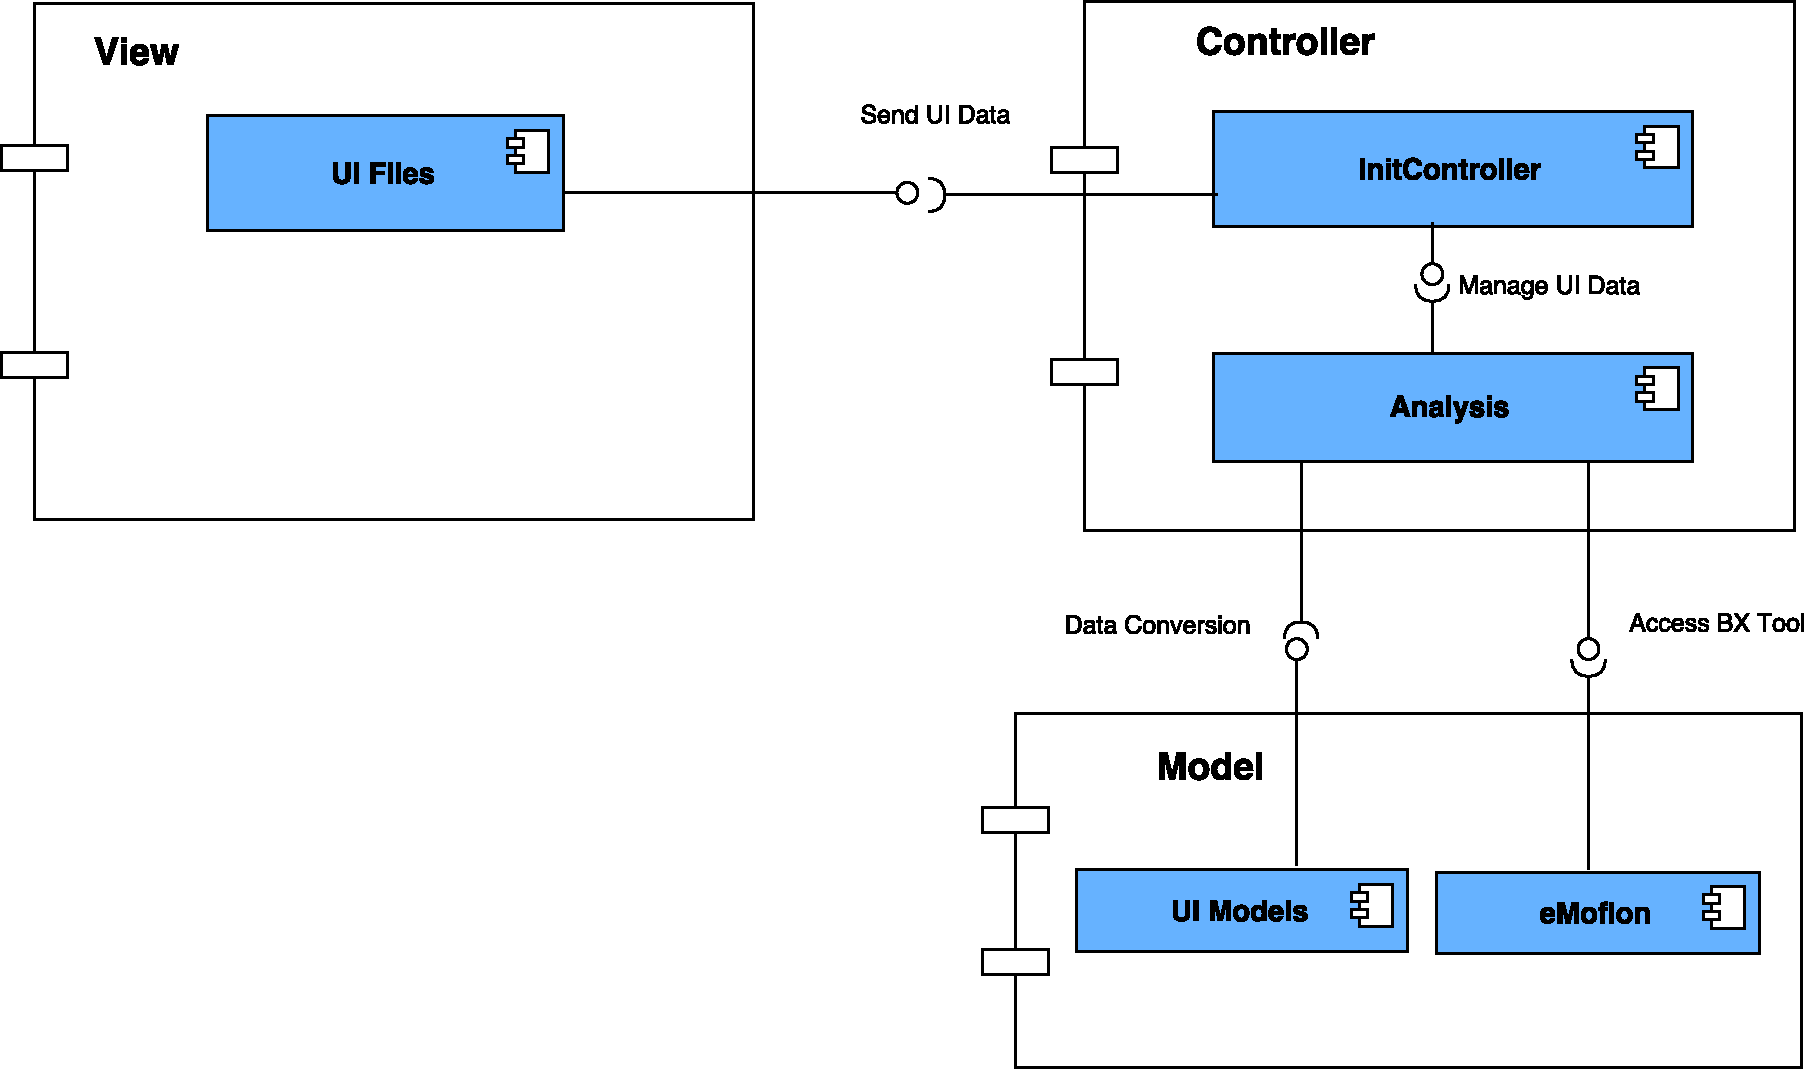
\includegraphics[width=1\textwidth]{figures/Component_Diagram}
	\caption{Component Diagram of Demon-BX Tool}
	\label{fig:Component_Diagram}
\end{sidewaysfigure}

On the top left, \texttt{View} component is present which contains a graphical user interface and functionalities that belong to the user. On the top right, \texttt{Controller} component is present which acts a bridge between view and model and processes all user requests. \texttt{Model} component is present at the below which contains the bx tool  and all transformation logic.

The \texttt{View} component is basically present in a web browser. It consist of the technologies like \texttt{HTML}, \texttt{CSS}, \texttt{JavaScript}, \texttt{Fabricjs} and \texttt{JQuery}. As a component, it is shown on a web browser as a part of a web application, provides an interface for a user to interact, and responsible for capturing all user related actions.

The \texttt{Controller} component is consist of a servlet i.e., \texttt{InitController} and a java class i.e., \texttt{Analysis}. \texttt{InitController} receives all the user requests sent from the web browser and calls the appropiate methods of the \texttt{Analysis} class where the actual data conversion happens, i.e., conversion of user data to model specific data before sending the them to the bx tool for further processing and conversion of model specific data to user data after receiving the data from the bx tool after processing.

The \texttt{Model} component consist of the \texttt{UI Models} i.e., java classes, bx tool i.e., \texttt{eMoflon}, and a few java classes encapsulating the implementation of the bx tool. It keeps all the models and transformation rules, processes the data send by the controller, and manages the state of all models along with its updated states. 

\subsubsection{General Workflow}\label{subsubsec:generalworkflow}
Figure~\ref{fig:Activity_Diagram} describes the general workflow of the Demon-BX tool in form of a activity diagram. The activity diagram basically provides an overview of the step by step actions performed by the tool. Detail workflow related to each layers will be described later in this document in Section \ref{subsec:imple_layers}.

\begin{figure}
	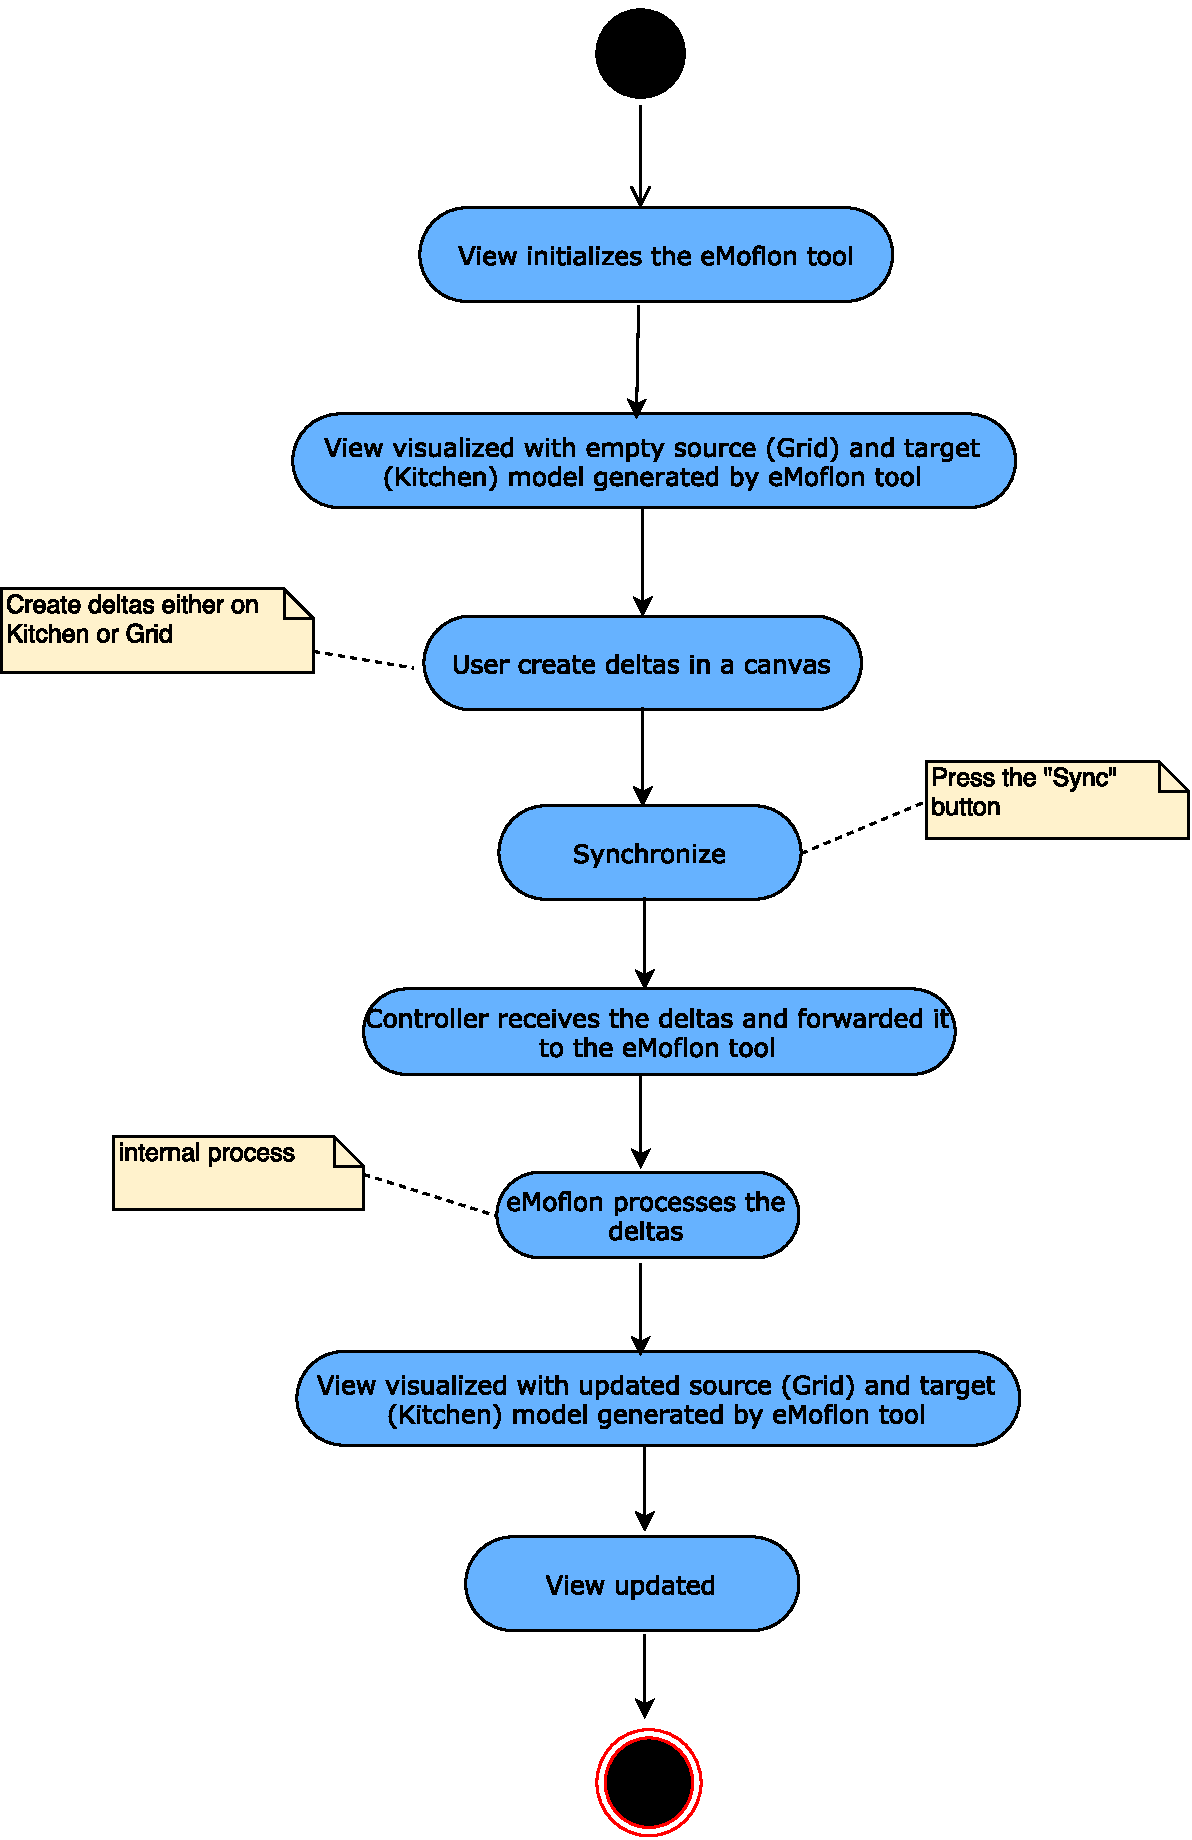
\includegraphics[width=0.8\textwidth]{figures/Activity_Diagram}
	\caption{Activity Diagram for General Workflow of Demon-BX Tool}
	\label{fig:Activity_Diagram}
\end{figure}

The first and foremost step is 'How to start the Demon-BX tool?'. As it is a web application, the user need to enter the complete URL of the tool on a web browser. As soon as the web page is loaded, it initializes the bx tool i.e., eMoflon. In return, the bx tool generates and sends a empty \texttt{Grid}, \texttt{Kitchen} model back to the web browser. After getting the empty models, view visualize them in two HTML canvas elements i.e., \texttt{Layout} and \texttt{Kitchen}. Then, user performs different actions on the canvas to create changes and press the \texttt{Sync} button to start the processing. These changes are collected and sent to the eMoflon tool for further processing. Once the processing is done, view receives the updated models from the tool and update both the canvas elements.

\subsubsection{Interaction between the Components}\label{subsubsec:componentinteraction}
Figure~\ref{fig:Sequence_Diagram} illustrates how the components introduced in Section \ref{subsubsec:component} interact with each other in the form of a sequence diagram. The sequence diagram especially shows an overview of the communication process between the components. Detail interaction of the layers and its inner components will be described later in this document in Section \ref{subsec:imple_layers}.

First, the user enters the URL and loads the web browser. As soon as the web browser is loaded, it sends an \texttt{Ajax} call i.e., \texttt{init} to the \texttt{Controller}. 

\begin{figure}
	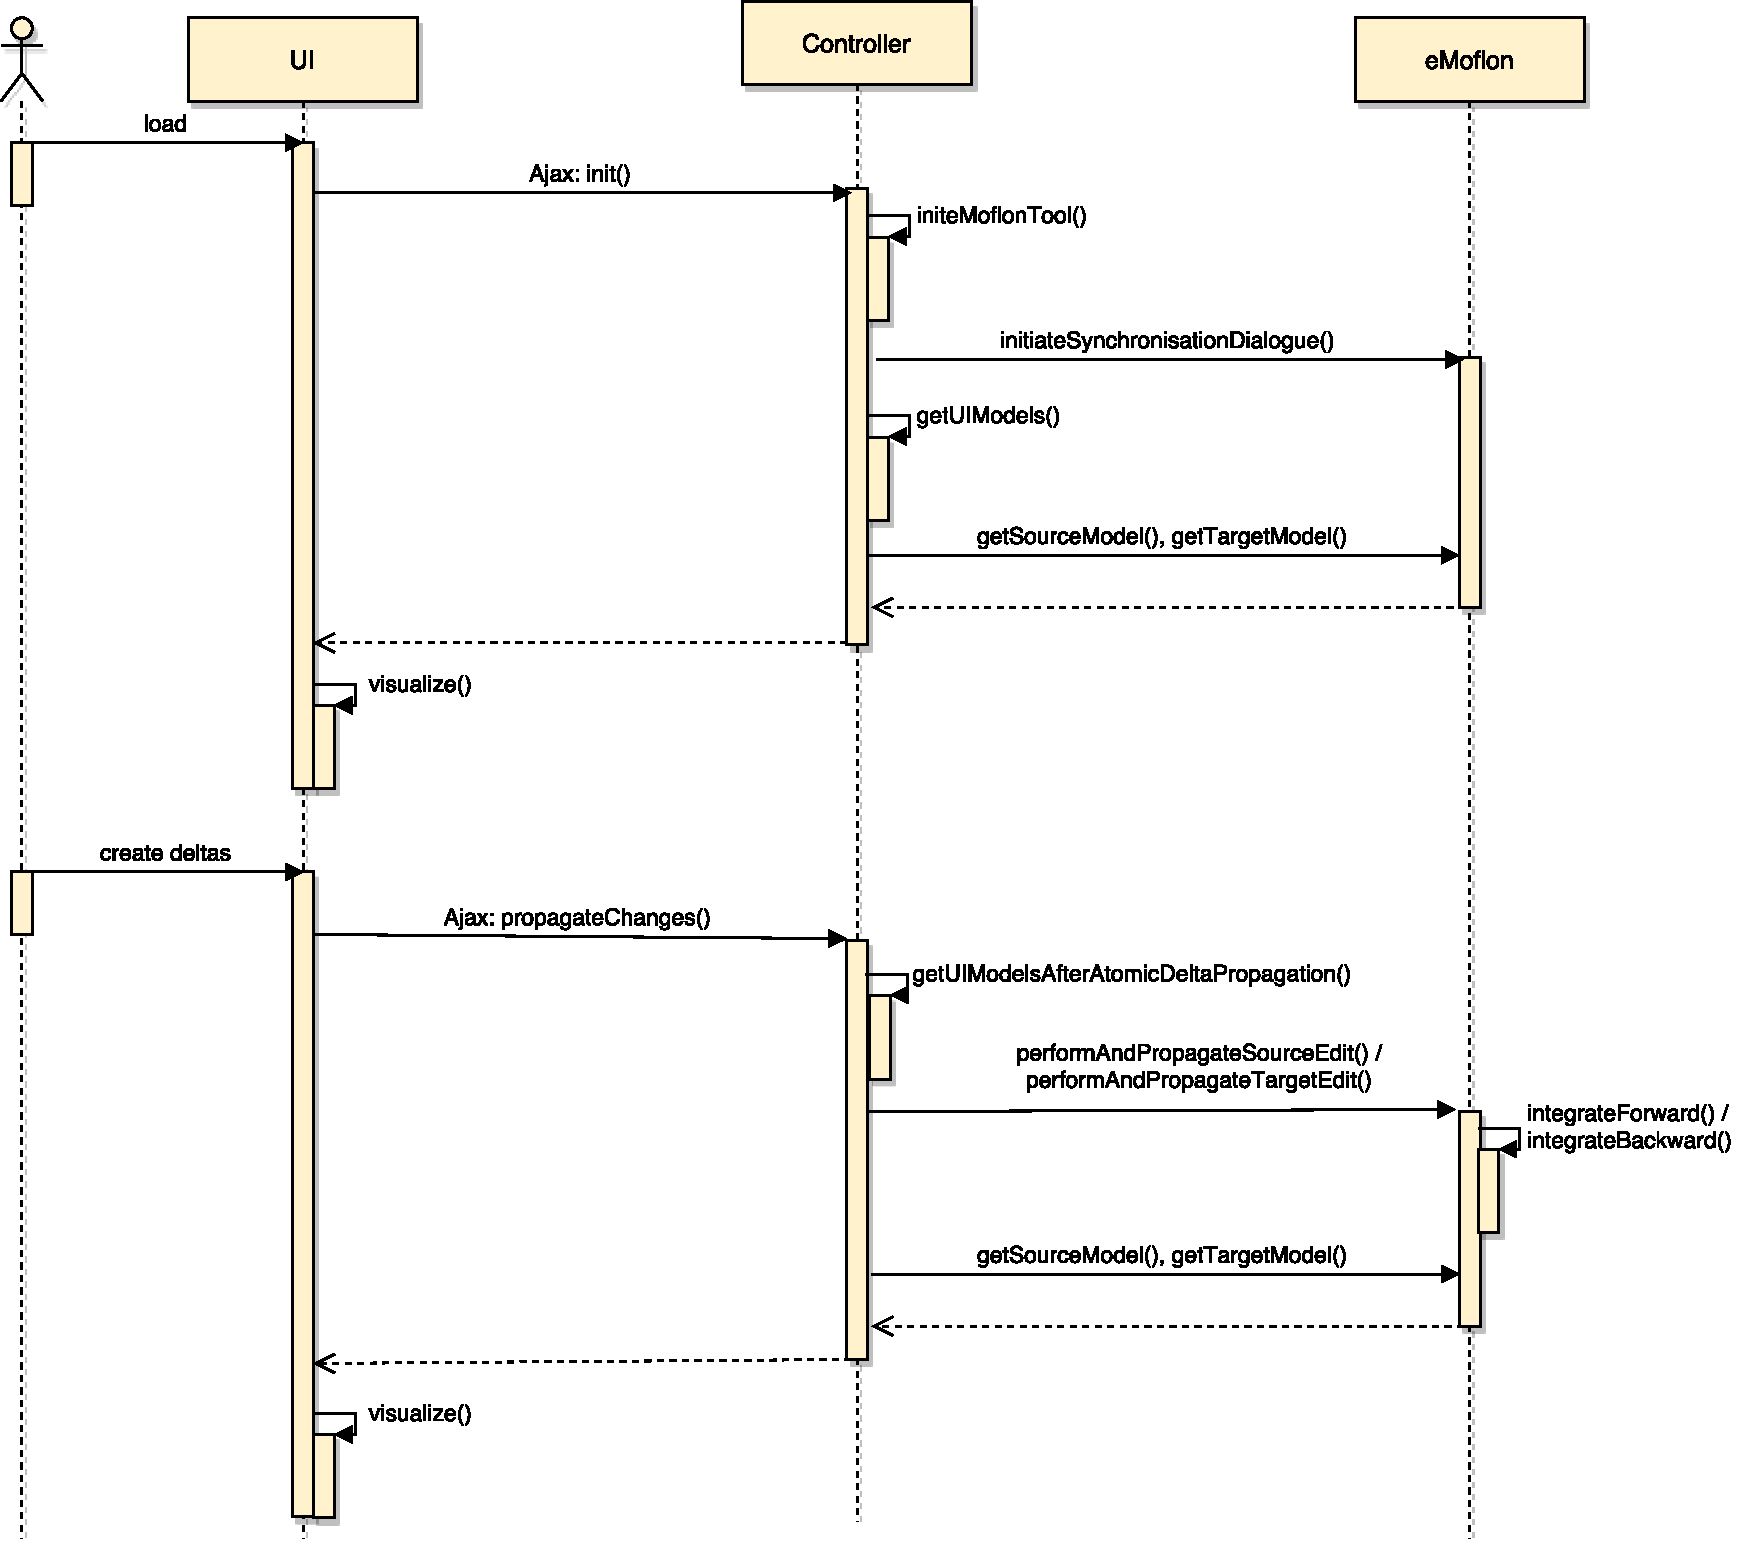
\includegraphics[width=1\textwidth]{figures/Sequence_Diagram}
	\caption{High Level Sequence Diagram of Demon-BX Tool}
	\label{fig:Sequence_Diagram}
\end{figure}

\subsection{Architecture Layers}\label{subsec:imple_layers}
This section describes each architecture layers i.e., Model, View, and Controller in detail from implementation point of view.

\subsubsection{Model}\label{subsubsec:imple_model}
\paragraph{Transformation Rules}

\subsubsection{View}\label{subsubsec:imple_view}

\begin{figure}
	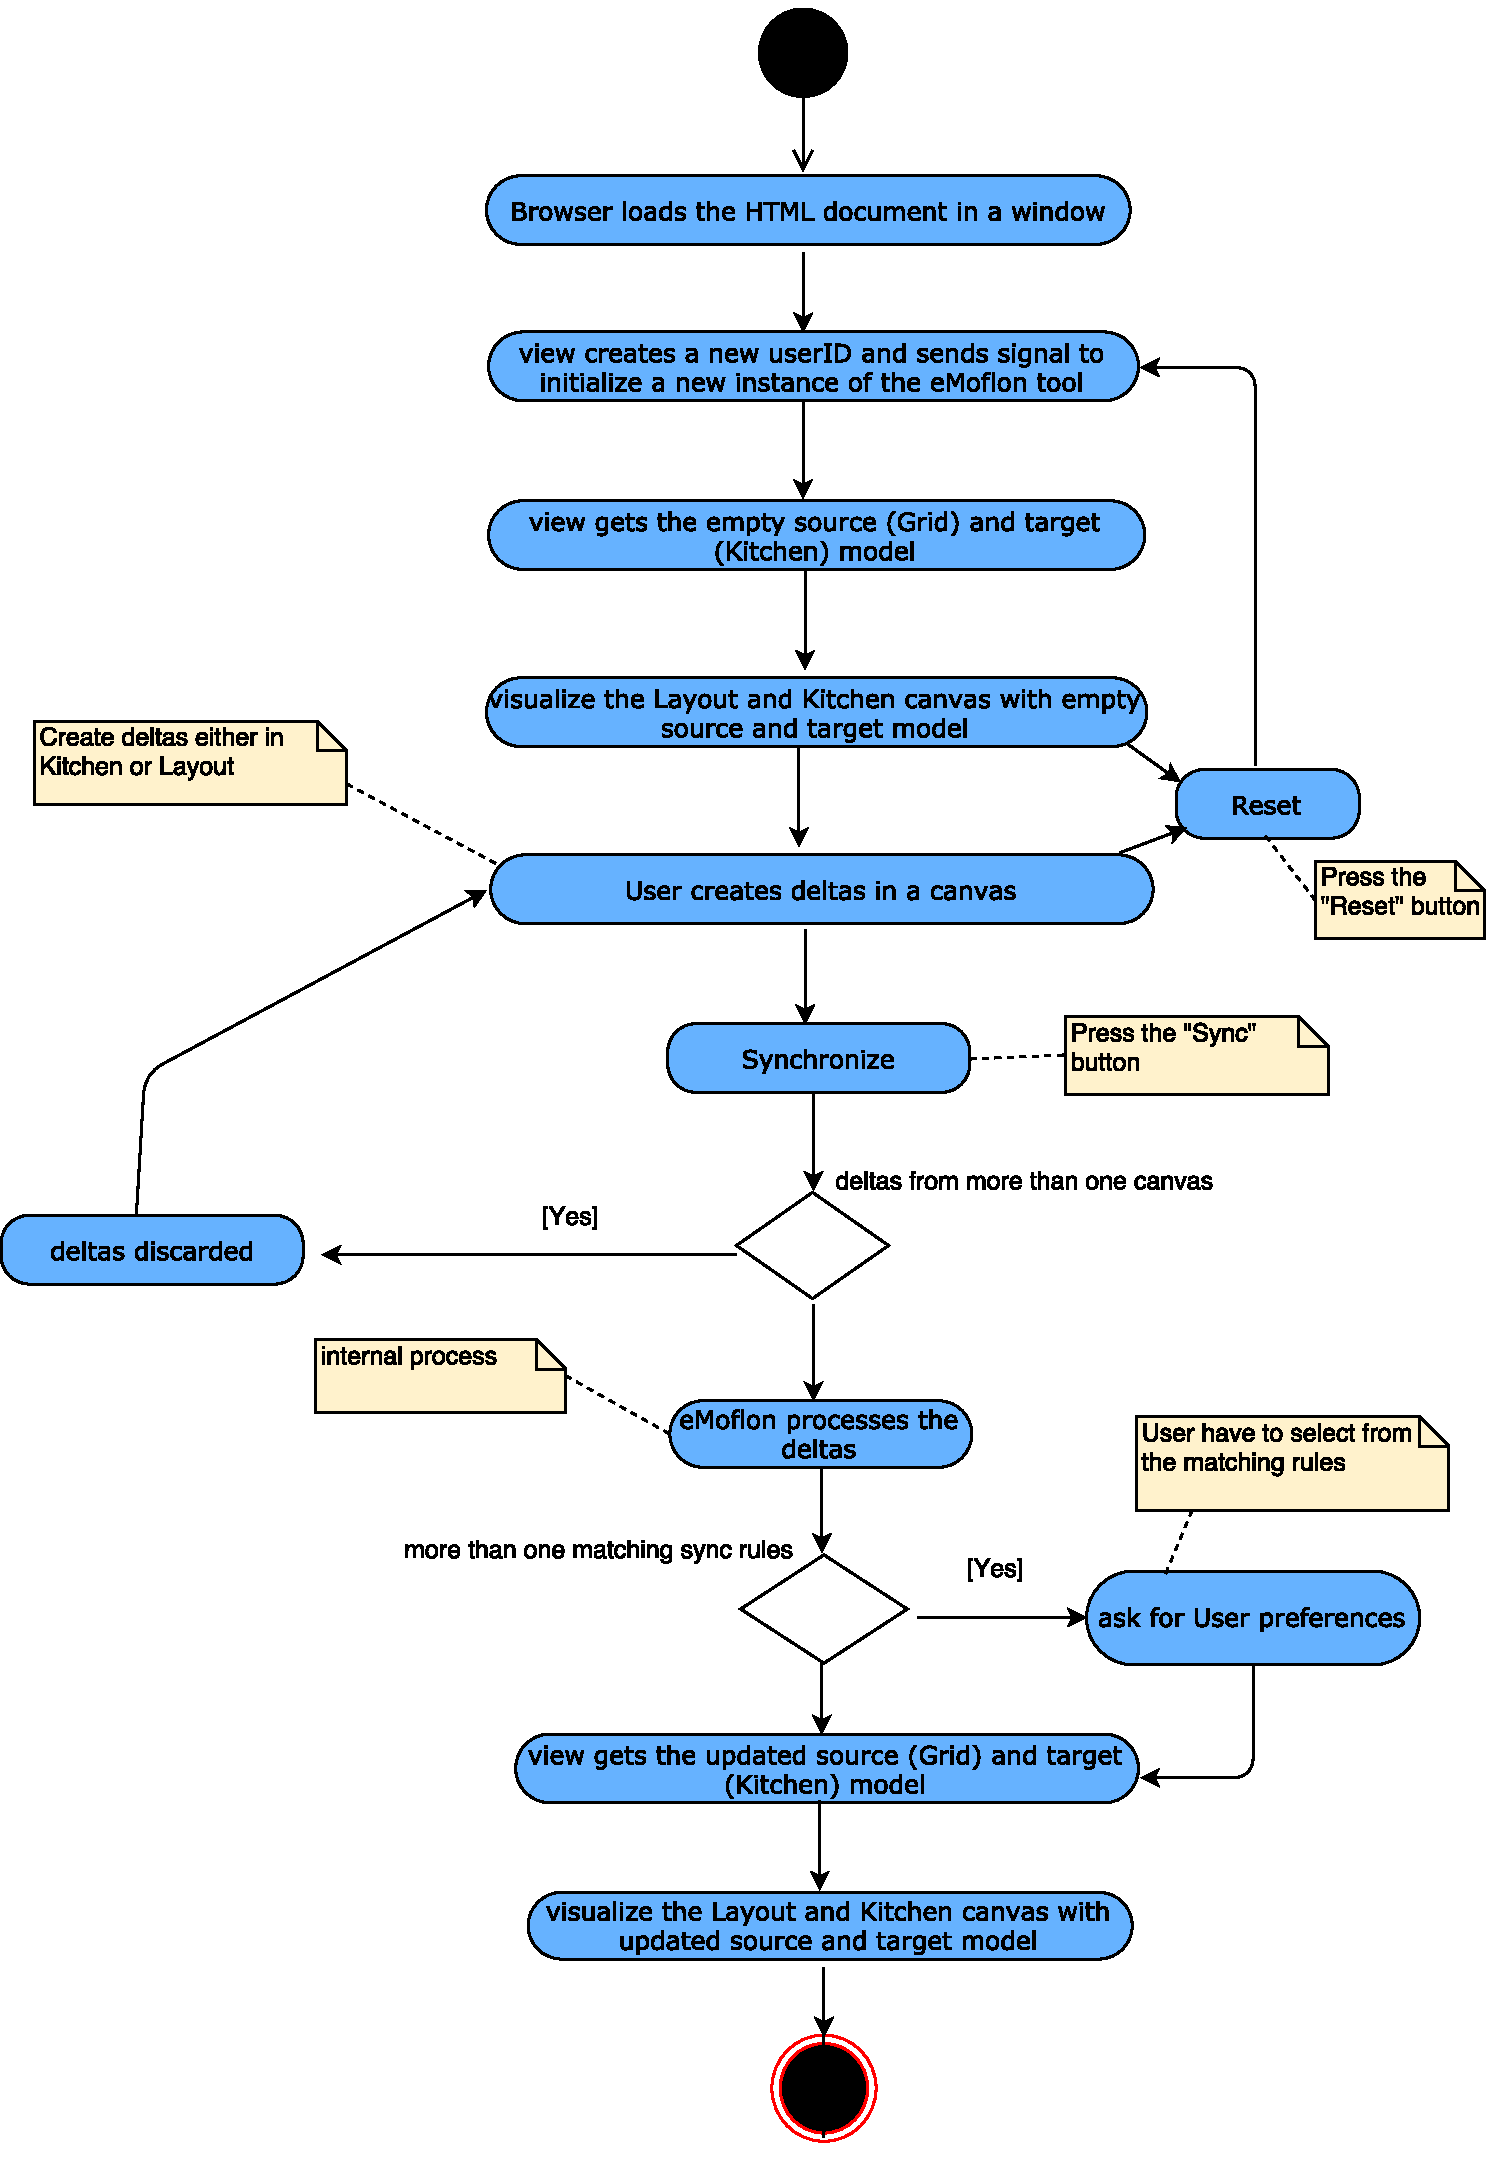
\includegraphics[width=0.9\textwidth]{figures/Activity_Diagram_View}
	\caption{Activity Diagram for View}
	\label{fig:Activity_Diagram_View}
\end{figure}

\subsubsection{Controller}\label{subsubsec:imple_controller}
controller and helper - how servlet is implemented with actual class name and func.

\subsection{Challenges}\label{subsec:implechallenges}
During the entire implementation process as explained in previous sections of this chapter, I came across a few challenges. This section describes them in detail.

\paragraph{Bx Tool}
selecting the type of delta (refer def.)
implementing atomic deltas to track successful/failed changes translation. 
User Choice Selection -- interupting the tool inbetween and start the process again

\paragraph{UI Implementation}
Designing the user interactions with high-level view was relatively easy as user have to deal with the objects with actions such as, mouse movements and button clicks. But, the real challenge was to handle the user interactions in low-level view's block structure. In low-level view, only addition and removal of objects are allowed and objects will be shown by unique colors. 

\paragraph{User Choice Selection}

\paragraph{Handling Multiple User Request}

\subsection{Choices and Threats}\label{subsec:imple_choicesthreats}
 



